\documentclass[aspectratio=169]{beamer}

% Load LongTREC theme (needs to be in same folder)
\usepackage{beamerthemeLongTREC}

% Extra TikZ/PGF libraries for advanced diagrams
\usetikzlibrary{arrows.meta, positioning, calc}
\usepackage{pgfplots}
\pgfplotsset{compat=1.18}
% Automatically handle image files with spaces or parentheses in their names
\usepackage{grffile}
% SVG inclusion support
\usepackage{svg}
% Bibliography support (biblatex with natbib compatibility)
\usepackage[style=authoryear,backend=biber]{biblatex}
\addbibresource{references.bib}

% Title information
\title{\texttt{SQANTI-reads}}
\subtitle{Quality assessment of long-read data in multi-sample lrRNA-seq experiments}
\author{Tianyuan Liu}
\institute{LongTREC Summer School 2025}
\date{\today}

% Remove vertical blue bar from Course Contents frame and keep numbered circles
\renewcommand{\tocframe}{%
  \begin{frame}
    \frametitle{Course Contents}
    \vspace{0.5em}
    {\setbeamertemplate{section in toc}{%
      % Align circle bullet baseline to the text baseline rather than the centre of the box
      \tikz[baseline=(num.base)] \node (num) [circle, fill=longtrec-blue, text=white, font=\bfseries, minimum size=1.1em, inner sep=0pt] {\inserttocsectionnumber};\hspace{0.8em}{\large\inserttocsection}\par%
    }%
    \setbeamertemplate{subsection in toc}{}%
    \tableofcontents[hideallsubsections]}%
  \end{frame}}

% Automatically insert the LongTREC themed section slide at every new section
% (title: current section name; subtitle left blank here).
\AtBeginSection{%
  \sectionframe{\insertsection}{}%
}

% Graphics path for external figure files
\graphicspath{{figures/}}

% Simple citation macro (manual)
\newcommand{\citep}[1]{(#1)}

% New math & table packages for PCA slides
\usepackage{amsmath, amsfonts, amssymb}
\usepackage{booktabs}

\begin{document}

% Title slide
\begin{frame}[plain]
  \titlepage
\end{frame}

% Contents slide
\tocframe

%%%%% SECTION: Background
\section{Background}

%--- Slide 1 -------------------------------------------------
\begin{frame}
  \frametitle{lrRNA-seq captures full-length transcripts}
  \begin{columns}[T]
    \begin{column}{0.55\textwidth}
      \begin{itemize}
        \item Long-read RNA sequencing directly sequences \textbf{full-length cDNA molecules}, preserving isoform structure \textsuperscript{[1]}.
      \end{itemize}
    \end{column}
    \begin{column}{0.4\textwidth}
      \centering
      % Actual schematic of a full-length transcript read
      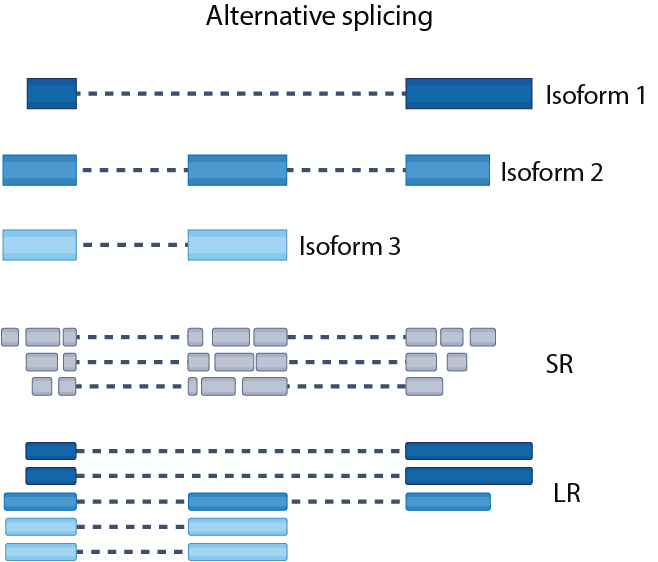
\includegraphics[width=0.9\linewidth]{Full-length_transcript_read.png}\\
      \vspace{0.2em}
      {\scriptsize\emph{Source:} \href{https://www.nature.com/articles/s41576-025-00828-z}{Monzó \emph{et al.}, 2025}}
    \end{column}
  \end{columns}
\end{frame}

%--- Slide 2 (Alternative Splicing) -------------------------------------------------
\begin{frame}
  \frametitle{lrRNA-seq reveals transcript diversity}
  \centering
  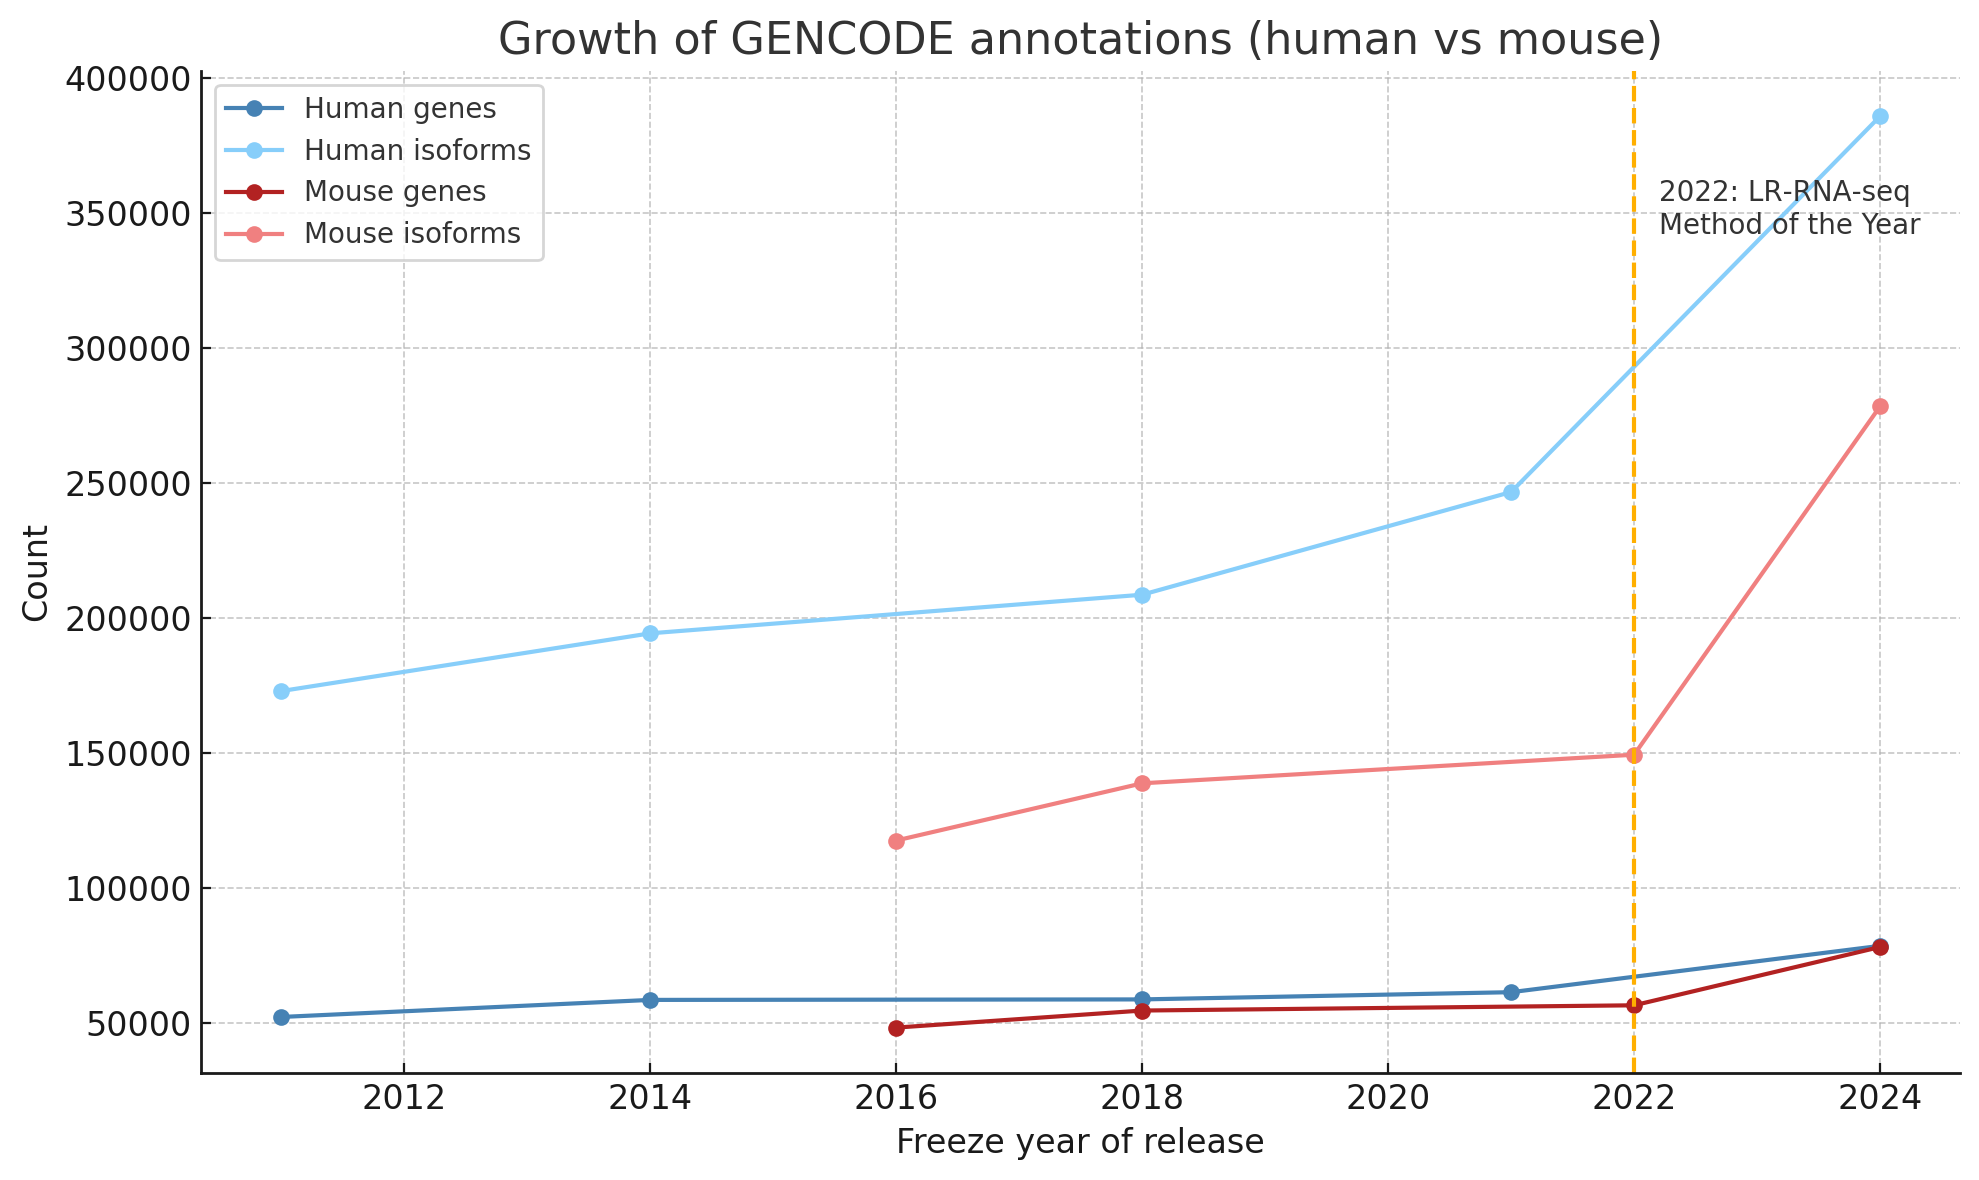
\includegraphics[width=0.78\textwidth]{Growth of GENCODE annotations (human vs mouse).png}\\
  % Source annotation for the plot
  \vspace{0.2em}
  {\scriptsize\emph{Source:} \href{https://www.gencodegenes.org/}{GENCODE} (Frankish \emph{et al.}, 2025)}
  \vspace{0.4em}
  \begin{itemize}
    \item Long-read sequencing enables comprehensive characterisation of \textbf{alternative splicing} and \textbf{transcript diversity} \textsuperscript{[5]}.
  \end{itemize}
\end{frame}

%--- Slide (Sources of error) -------------------------------------------------
\begin{frame}
  \frametitle{Sources of error in lrRNA-seq}
  \centering
  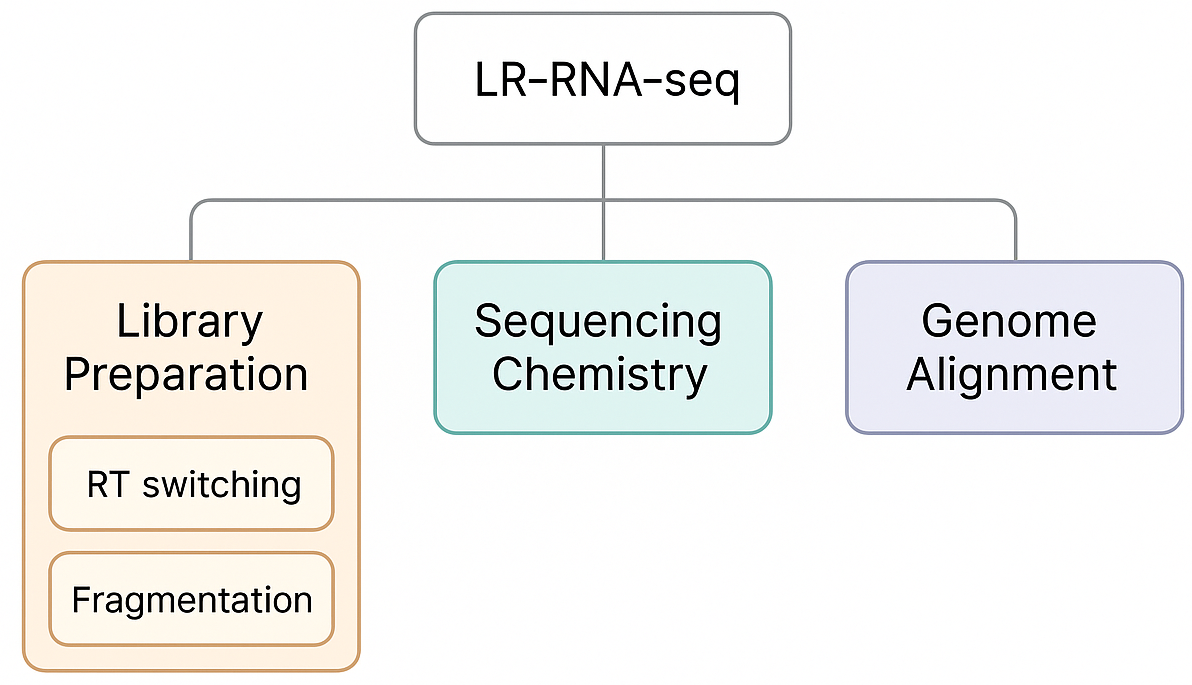
\includegraphics[width=0.7\textwidth]{lr-rna-seq_errors.png}\\
  \vspace{0.2em}
  {\scriptsize\emph{Errors: \textbf{library preparation} (RT switching, degradation), \textbf{sequencing chemistry}, or \textbf{genome alignment}.}}
\end{frame}

%--- New Slide: Reverse Transcriptase Template Switching (RT-switching) -----
\begin{frame}
  \frametitle{Reverse Transcriptase Template Switching (RT-switching)}
  \begin{columns}[T]
    \begin{column}{0.6\textwidth}
      \centering
      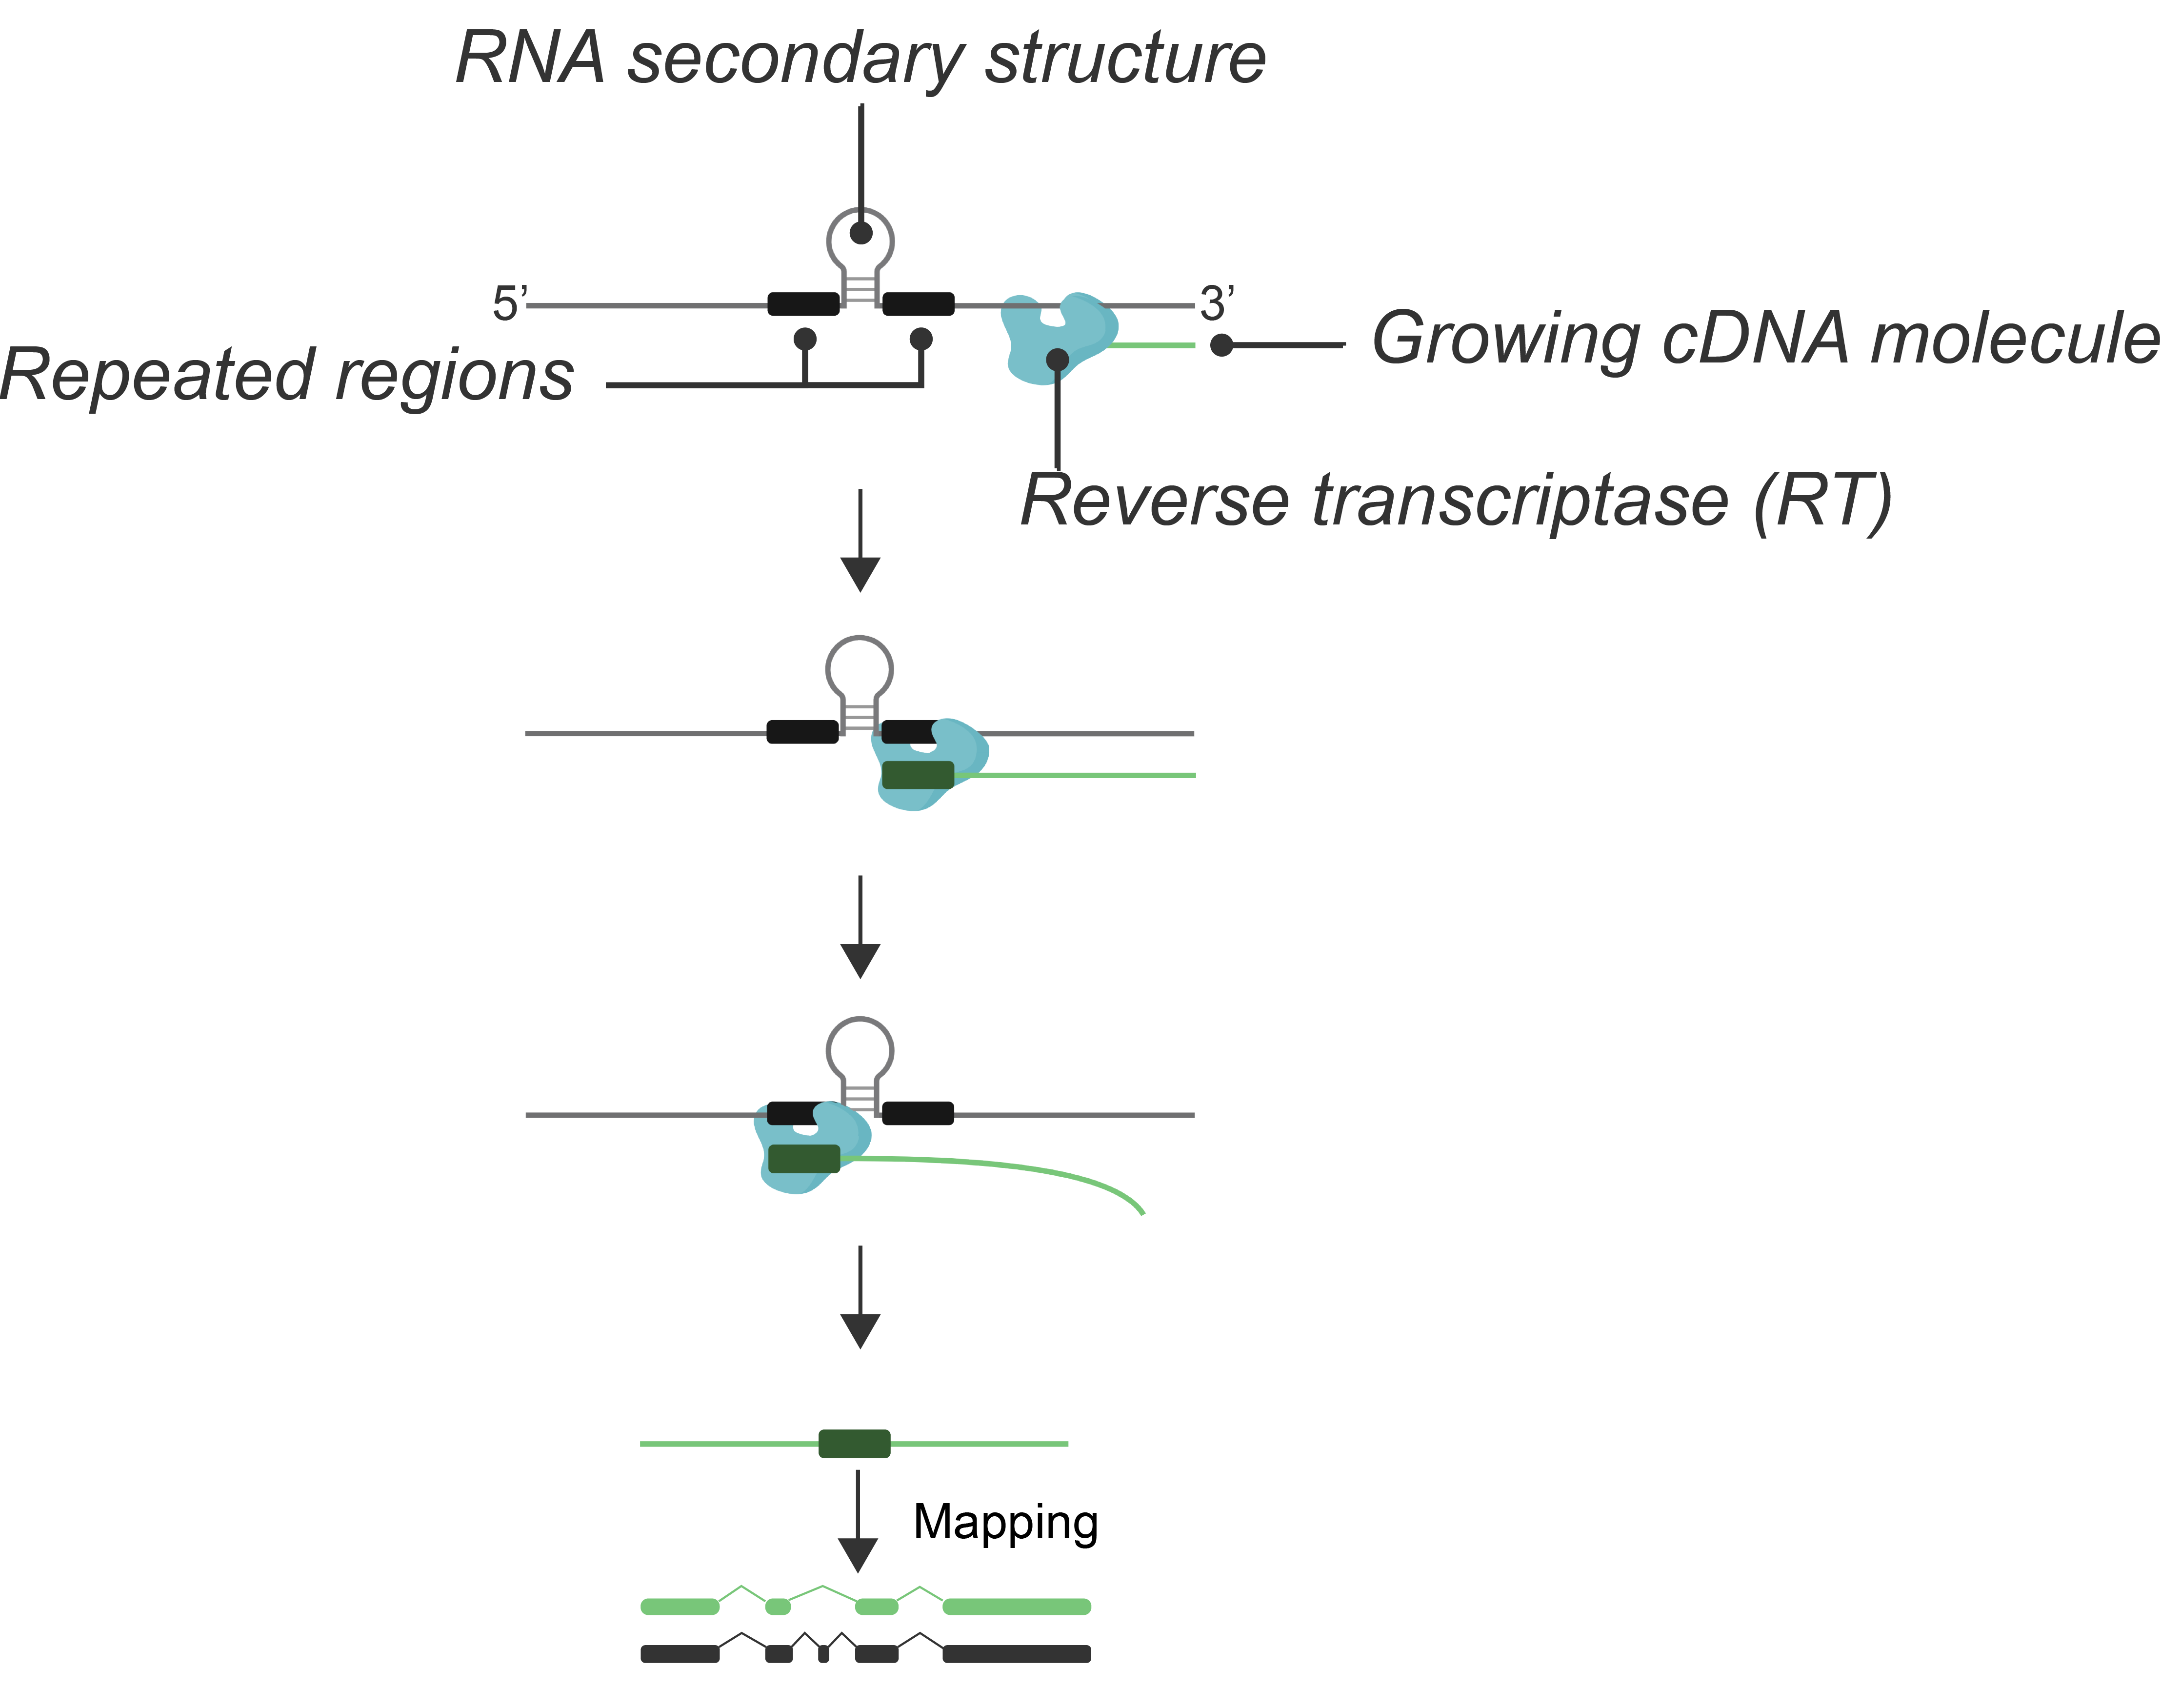
\includegraphics[width=\textwidth]{rt-switching.png}
    \end{column}
    \begin{column}{0.35\textwidth}
      \small
      RT enzyme can "jump" between templates at repeated regions, creating chimeric cDNA products that confound transcript analysis.
    \end{column}
  \end{columns}
\end{frame}

%--- New Slide: Intra-priming -----------------------------------------------
\begin{frame}
  \frametitle{Intra-priming}
  \centering
  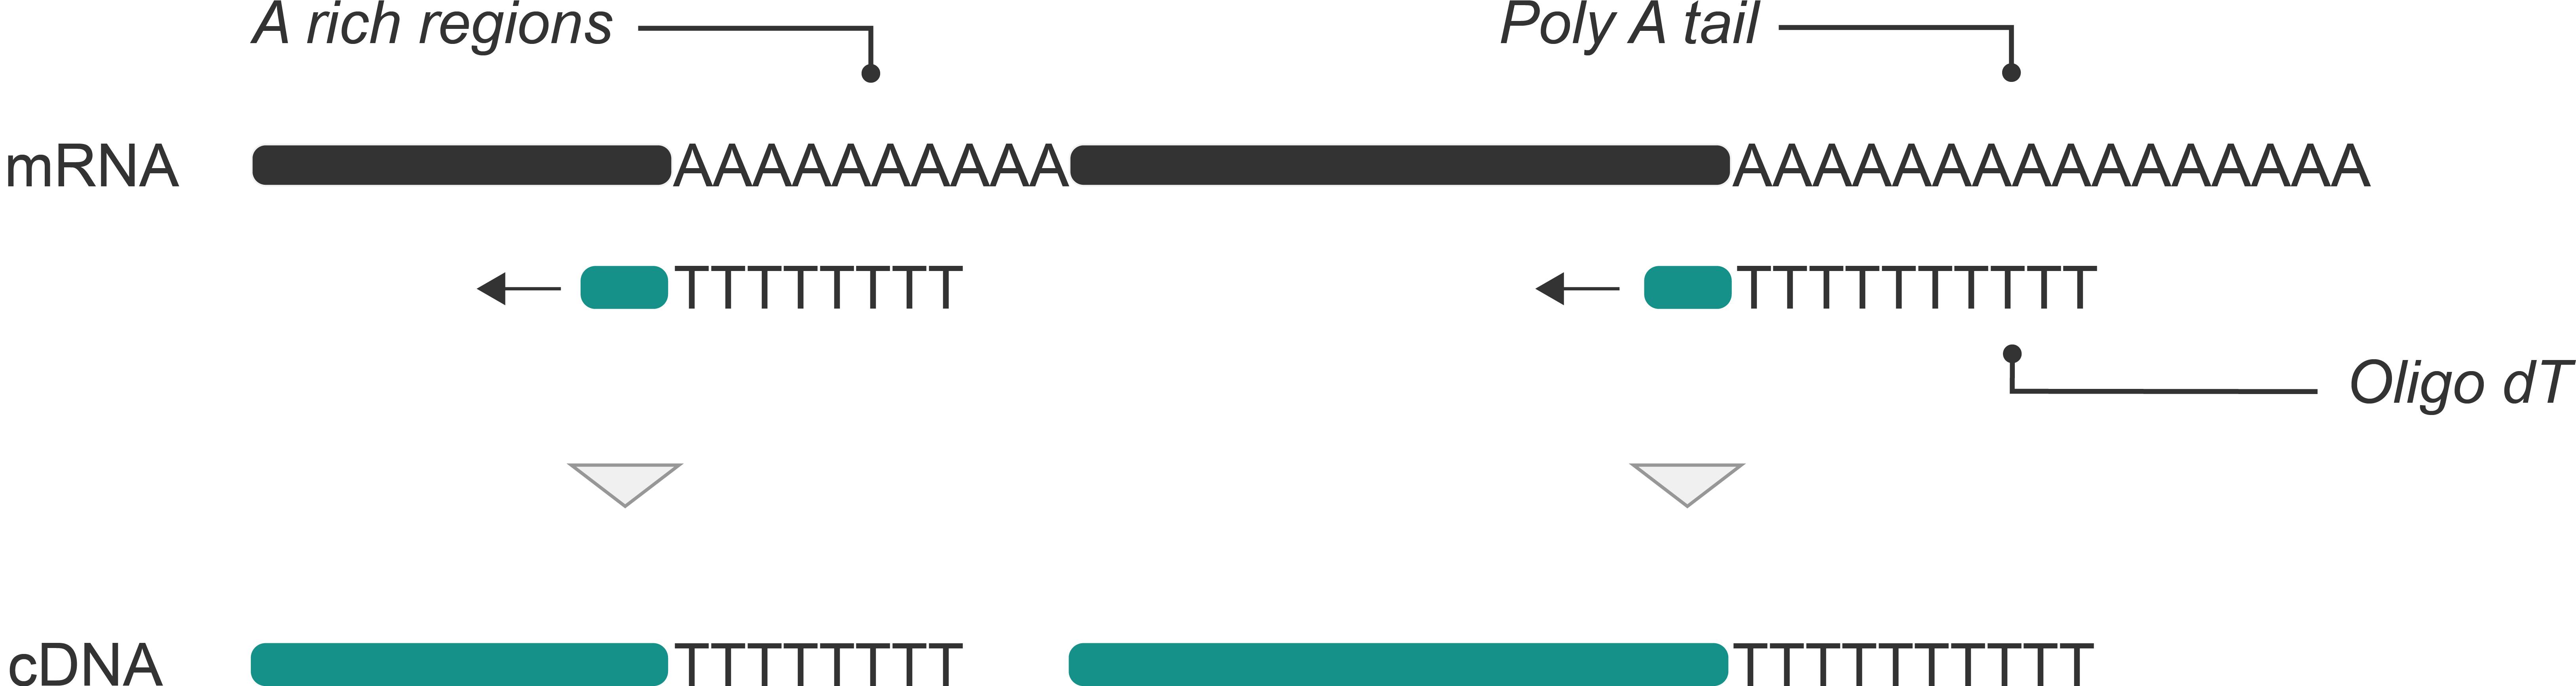
\includegraphics[width=0.8\textwidth]{intra-priming.png}
  
  \vspace{0.5cm}
  
  \small
  Oligo-dT primers can bind to internal A-rich regions, causing truncated cDNA synthesis.
\end{frame}

%--- Slide 3&4 (combined) -----------------------------------
\begin{frame}
  \frametitle{QC in lrRNA-seq: Importance \& Current Limitations}
  \begin{columns}[T]
    \begin{column}{0.9\textwidth}
      \begin{block}{Why rigorous QC is essential}
        \begin{itemize}
          \item QC filters problematic reads, ensuring reliable downstream \textbf{quantification} and \textbf{novel isoform discovery} \textsuperscript{[3]}.
          \item Facilitates cross-sample comparison and prevents confounding technical artefacts.
        \end{itemize}
      \end{block}
      \vspace{0.4cm}
      \begin{block}{Limitations of traditional QC tools}
        \begin{itemize}
          \item Most QC tools evaluate \textbf{read-level metrics} (length, Phred quality) but overlook \textbf{transcript structure}. 
          \item Structural context is key for identifying mis-spliced or truncated reads \textsuperscript{[4]}.
        \end{itemize}
      \end{block}
    \end{column}
  \end{columns}
\end{frame}

%--- Check-in Questions: Background ----------------------------------------
\begin{frame}
  \frametitle{Check-in Questions: Background}
  \begin{enumerate}
    \item What are the main advantages of long-read RNA sequencing over short-read sequencing for transcript analysis?
    \vspace{0.5cm}
    \item Can you name two major sources of error that can occur during lrRNA-seq library preparation?
  \end{enumerate}
\end{frame}

%%%%% SECTION: Introducing \texttt{SQANTI-reads}
\section{Introducing \texttt{SQANTI-reads}}

\begin{frame}
  \frametitle{What is \texttt{SQANTI-reads}?}
  \begin{columns}[T]
    \begin{column}{0.58\textwidth}
      \begin{block}{\textbf{A read-centric extension of SQANTI3}}
        \begin{itemize}
          \item Ports \textbf{SQANTI3} structural classification to the \textbf{single-read} level.
          \item Jointly evaluates \emph{raw reads} from \textbf{multiple samples} in one run.
          \item Summarises structural categories, splicing patterns, and junction usage.
          \item Produces \emph{interactive} visualisations to spot outliers and under-annotated genes.
        \end{itemize}
      \end{block}
    \end{column}
    \begin{column}{0.38\textwidth}
      % Compact vertical pipeline schematic with multiple samples
      \hspace*{-0.45cm}% left shift
      \begin{tikzpicture}[node distance=0.5cm and 0.25cm,
          box/.style={draw, rounded corners=1pt, fill=longtrec-lightgray, font=\scriptsize, align=center, inner sep=3pt, minimum width=2.5cm},
          sample/.style={draw, rounded corners=1pt, fill=longtrec-lightgray, font=\scriptsize, align=center, inner sep=2pt, minimum width=2cm},
          arrow/.style={-Stealth, thick, color=longtrec-blue},
          every node/.style={transform shape}]
        % Sample nodes (top row)
        \node (raw1) [sample] {Sample~1\\Reads};
        \node (raw2) [sample, right=of raw1] {Sample~2\\Reads};
        \node (raw3) [sample, right=of raw2] {Sample~3\\Reads};
        % Downstream nodes
        \node (aln) [box, below=of raw2] {Genome\\Alignment\\(\texttt{minimap2})};
        \node (cls) [box, below=of aln] {SQANTI3\\Structural\\Category};
        \node (met) [box, below=of cls] {Read\\Metrics};
        \node (rep) [box, fill=longtrec-orange!50, below=of met] {Interactive\\Report};
        % Arrows from samples to alignment
        \draw[arrow] (raw1) -- (aln);
        \draw[arrow] (raw2) -- (aln);
        \draw[arrow] (raw3) -- (aln);
        % Vertical arrows downstream
        \draw[arrow] (aln) -- (cls);
        \draw[arrow] (cls) -- (met);
        \draw[arrow] (met) -- (rep);
      \end{tikzpicture}
    \end{column}
  \end{columns}
\end{frame}

%--- New Slide: Inputs & Outputs ---------------------------------
\begin{frame}
  \frametitle{\texttt{SQANTI-reads}: Inputs \& Outputs}
  \begin{columns}[T]
    \begin{column}{0.48\textwidth}
      \textbf{Core Inputs}
      \begin{itemize}
        \item \textbf{Design file (CSV)} – columns \texttt{sampleID}, \texttt{file\_acc}.
        \item \textbf{Reference annotation} (GTF/GFF3).
      \end{itemize}
      \vspace{0.3em}
      \textbf{Mode\,–\,dependent}
      \begin{itemize}
        \item \emph{Fast mode:} pre-computed SQANTI3-QC output directories\\(given via \texttt{--input\_dir}).
        \item \emph{Simple mode:} raw reads (\texttt{*.fastq}) or sample GTF/GFF\\\phantom{---}+ reference genome FASTA.
      \end{itemize}
      \vspace{0.3em}
    \end{column}
    \begin{column}{0.48\textwidth}
      \textbf{Key Outputs}
      \begin{itemize}
        \item Modified \texttt{reads\_classification.txt} (adds \texttt{jxn\_string}, \texttt{jxnHash}).
        \item Updated \texttt{design.csv} (adds \texttt{classification\_file}, \texttt{junction\_file}).
        \item Summary CSV tables: gene\_counts, ujc\_counts, length\_summary, cv, etc.
        \item QC plots PDF (default) \emph{\&} optional HTML report.
        \item Annotation plots PDF.
      \end{itemize}
      \vspace{0.3em}
    \end{column}
  \end{columns}
  \vspace{0.15cm}
\end{frame}

%--- New Slide: Genomic Features ---------------------------------
\begin{frame}
  \frametitle{Structure of a eukaryotic gene}
  \centering
  % Display only the gene schematic (TikZ)
  \begin{tikzpicture}[font=\scriptsize, >=Stealth]
    % Coordinate definitions
    \def\utr{0.8}
    \def\ex{2.0}
    \def\intr{1.0}
    \def\height{0.5}
    % 5' UTR
    \draw[fill=longtrec-blue, draw=none] (0,0) rectangle (\utr,\height);
    % Exon 1
    \draw[fill=longtrec-orange, draw=none] (\utr,0) rectangle (\utr+\ex,\height);
    % Intron 1
    \draw[fill=longtrec-lightgray!50, draw=none] (\utr+\ex,0) rectangle (\utr+\ex+\intr,\height);
    % Exon 2
    \draw[fill=longtrec-orange, draw=none] (\utr+\ex+\intr,0) rectangle (\utr+2*\ex+\intr,\height);
    % Intron 2
    \draw[fill=longtrec-lightgray!50, draw=none] (\utr+2*\ex+\intr,0) rectangle (\utr+2*\ex+2*\intr,\height);
    % Exon 3
    \draw[fill=longtrec-orange, draw=none] (\utr+2*\ex+2*\intr,0) rectangle (\utr+3*\ex+2*\intr,\height);
    % 3' UTR
    \draw[fill=longtrec-blue, draw=none] (\utr+3*\ex+2*\intr,0) rectangle (\utr+3*\ex+2*\intr+\utr,\height);

    % Flanking lines extending beyond UTRs
    \def\flank{0.8}
    \draw[longtrec-blue, line width=0.8pt] (-\flank,0.25) -- (0,0.25);
    \draw[longtrec-blue, line width=0.8pt] (\utr+3*\ex+2*\intr+\utr,0.25) -- (\utr+3*\ex+2*\intr+\utr+\flank,0.25);

    % Promoter arrow: point upward toward gene line, label below arrow tail
    \def\promX{-0.6}
    \draw[->] (\promX,-0.45) -- (\promX,0.25);
    \node[below=2pt] at (\promX,-0.45) {Promoter region};

    % Downward arrows & labels for introns (top)
    \def\arrowTop{1.2}
    % Intron 1 (raise label above the gene)
    \draw[->] (\utr+\ex+0.5*\intr,\arrowTop) node[above=8pt] {Intron 1} -- (\utr+\ex+0.5*\intr,0.25);
    % Intron 2 (raise label)
    \draw[->] (\utr+2*\ex+1.5*\intr,\arrowTop) node[above=8pt] {Intron 2} -- (\utr+2*\ex+1.5*\intr,0.25);

    % Downward arrows & labels for UTRs (top)
    % 5' UTR (raise label)
    \draw[->] (0.5*\utr,\arrowTop) node[above=8pt] {$5'$ UTR} -- (0.5*\utr,0.25);
    % 3' UTR (raise label)
    \draw[->] (\utr+3*\ex+2*\intr+0.5*\utr,\arrowTop) node[above=8pt] {$3'$ UTR} -- (\utr+3*\ex+2*\intr+0.5*\utr,0.25);

    % Labels inside exons
    \node at (\utr+0.5*\ex,0.25) {Exon 1};
    \node at (\utr+\ex+\intr+0.5*\ex,0.25) {Exon 2};
    \node at (\utr+2*\ex+2*\intr+0.5*\ex,0.25) {Exon 3};
    % Further separate the 5' and 3' labels horizontally
    \def\labY{0.6}
    \node[anchor=east] at (-0.5,\labY) {$5'$};
    \node[anchor=west] at (\utr+3*\ex+2*\intr+\utr+0.7,\labY) {$3'$};
  \end{tikzpicture}
  \vspace{0.3cm}
  \vspace{0.3cm}
  {\scriptsize\emph{Schematic of a canonical eukaryotic gene: promoter (blue), untranslated regions, coding exons (orange), introns (grey), and transcriptional orientation from $5'$ to $3'$.}}
  \vspace{0.3cm}
\end{frame}

% Slide 1: conceptual differences
\begin{frame}
  \frametitle{GTF vs GFF3: Key Differences}
  \begin{itemize}
    \item Both share the first eight columns: \texttt{seqid, source, type, start, end, score, strand, phase}.
    \item \textbf{Attribute syntax}
      \begin{itemize}
        \item \textbf{GTF}: \texttt{<key> "value";} (semicolon-terminated key–value pairs).
        \item \textbf{GFF3}: \texttt{key=value} (comma-separated if multiple) with \texttt{ID} / \texttt{Parent} tags enabling feature hierarchies.
      \end{itemize}
    \item \textbf{Specification status}: GTF is legacy (GFF2-derived); GFF3 is the current, more flexible standard.
  \end{itemize}
\end{frame}

% Slide 2: example records illustrating the differences
\begin{frame}[fragile]
  \frametitle{Example Records: GTF vs GFF3}
  {\tiny
  \textbf{GTF}\vspace{0.2em}\\
\begin{verbatim}
chr1 HAVANA gene            11869 14409 . + . gene_id "ENSG00000223972";
chr1 HAVANA transcript      11869 14409 . + . gene_id "ENSG00000223972"; transcript_id "ENST00000456328";
chr1 HAVANA exon            11869 12227 . + . gene_id "ENSG00000223972"; transcript_id "ENST00000456328"; exon_number "1";
chr1 HAVANA five_prime_UTR  11869 12009 . + . gene_id "ENSG00000223972"; transcript_id "ENST00000456328";
chr1 HAVANA CDS             12010 12057 . + 0 gene_id "ENSG00000223972"; transcript_id "ENST00000456328";
chr1 HAVANA three_prime_UTR 12058 14409 . + . gene_id "ENSG00000223972"; transcript_id "ENST00000456328";
\end{verbatim}
  \vspace{0.4em}
  \textbf{GFF3}\vspace{0.2em}\\
\begin{verbatim}
chr1 HAVANA gene            11869 14409 . + . ID=gene0;Name=DDX11L1;
chr1 HAVANA transcript      11869 14409 . + . ID=transcript0;Parent=gene0;
chr1 HAVANA exon            11869 12227 . + . ID=exon0;Parent=transcript0;
chr1 HAVANA five_prime_UTR  11869 12009 . + . ID=futr0;Parent=transcript0;
chr1 HAVANA CDS             12010 12057 . + 0 ID=cds0;Parent=transcript0;
chr1 HAVANA three_prime_UTR 12058 14409 . + . ID=tutr0;Parent=transcript0;
\end{verbatim}}
\end{frame}

%--- Key Features: Unique Junction Chain ---------------------------------
\begin{frame}
  \frametitle{Key Features: Unique Junction Chain}
  \centering
  \makebox[\textwidth]{%
  \begin{tikzpicture}[scale=1.15,
      exon/.style={draw, fill=longtrec-blue!50, minimum height=4pt, inner sep=0pt},
      intron/.style={thick, draw=longtrec-blue},
      arrow/.style={-Stealth, thick, color=longtrec-orange},
      every node/.style={font=\scriptsize}]
    % ------------ Reads with variable TSS/TTS but identical internal junctions ------------
    \def\xA{0}  % unified start
    \def\xB{1.4}
    \def\xC{2.8}
    \def\xD{4.2}
    % Read 1 (top) – canonical exon lengths
    \draw[exon] (\xA,0)      rectangle ++(1,0.25);
    \draw[exon] (\xB,0)      rectangle ++(1,0.25);
    \draw[exon] (\xC,0)      rectangle ++(1,0.25);
    \draw[exon] (\xD,0)      rectangle ++(1,0.25);
    \draw[intron] (\xA+1,0.125) .. controls +(0.25,0.4) and +(-0.25,0.4) .. (\xB,0.125);
    \draw[intron] (\xB+1,0.125) .. controls +(0.25,0.4) and +(-0.25,0.4) .. (\xC,0.125);
    \draw[intron] (\xC+1,0.125) .. controls +(0.25,0.4) and +(-0.25,0.4) .. (\xD,0.125);
    \node[anchor=east] at (\xA-0.5,0.125) {\scriptsize Read~1};
    % Read 2 (middle) – unchanged TSS, longer TTS
    \draw[exon] (\xA-0.3,-0.7) rectangle ++(1.3,0.25); % longer TSS
    \draw[exon] (\xB,-0.7)   rectangle ++(1,0.25);
    \draw[exon] (\xC,-0.7)   rectangle ++(1,0.25);
    \draw[exon] (\xD,-0.7)   rectangle ++(1.3,0.25);
    \draw[intron] (1,-0.575) .. controls +(0.25,0.4) and +(-0.25,0.4) .. (\xB,-0.575);
    \draw[intron] (\xB+1,-0.575) .. controls +(0.25,0.4) and +(-0.25,0.4) .. (\xC,-0.575);
    \draw[intron] (\xC+1,-0.575) .. controls +(0.25,0.4) and +(-0.25,0.4) .. (\xD,-0.575);
    \node[anchor=east] at (\xA-0.5,-0.575) {\scriptsize Read~2};
    % Read 3 (bottom) – unchanged TSS, shorter TTS
    \draw[exon] (\xA+0.2,-1.4) rectangle ++(0.8,0.25); % shorter TSS
    \draw[exon] (\xB,-1.4)   rectangle ++(1,0.25);
    \draw[exon] (\xC,-1.4)   rectangle ++(1,0.25);
    \draw[exon] (\xD,-1.4)   rectangle ++(0.7,0.25);
    \draw[intron] (1,-1.275) .. controls +(0.25,0.4) and +(-0.25,0.4) .. (\xB,-1.275);
    \draw[intron] (\xB+1,-1.275) .. controls +(0.25,0.4) and +(-0.25,0.4) .. (\xC,-1.275);
    \draw[intron] (\xC+1,-1.275) .. controls +(0.25,0.4) and +(-0.25,0.4) .. (\xD,-1.275);
    \node[anchor=east] at (\xA-0.5,-1.275) {\scriptsize Read~3};

    % Curly brace grouping the reads (shifted right)
    \draw[decorate,decoration={brace, amplitude=4pt}, thick] (\xD+1.6,0.18) -- (\xD+1.6,-1.42) node[midway,right=4pt,font=\scriptsize] {Same junction chain};

    % Arrow leading to collapsed UJC representation
    \draw[arrow, thick] (\xB+0.5,-1.55) -- (\xB+0.5,-1.9);

    % ------------ Collapsed Unique Junction Chain (shows all three junctions) ------------
    \draw[exon, fill=longtrec-orange!50] (\xA,-2.3)   rectangle ++(1,0.25);
    \draw[exon, fill=longtrec-orange!50] (\xB,-2.3)   rectangle ++(1,0.25);
    \draw[exon, fill=longtrec-orange!50] (\xC,-2.3)   rectangle ++(1,0.25);
    \draw[exon, fill=longtrec-orange!50] (\xD,-2.3)   rectangle ++(1,0.25);
    % three introns for UJC (match read arcs)
    \draw[intron, draw=longtrec-orange!60] (\xA+1,-2.175) .. controls +(0.25,0.35) and +(-0.25,0.35) .. (\xB,-2.175);
    \draw[intron, draw=longtrec-orange!60] (\xB+1,-2.175) .. controls +(0.25,0.35) and +(-0.25,0.35) .. (\xC,-2.175);
    \draw[intron, draw=longtrec-orange!60] (\xC+1,-2.175) .. controls +(0.25,0.35) and +(-0.25,0.35) .. (\xD,-2.175);
    % annotation & label
    \node[anchor=east] at (\xA-0.5,-2.175) {\scriptsize UJC};
    \node[font=\scriptsize, align=center] at (\xB+0.5,-3.1) {Reads have variable TSS/TTS but share the same ordered splice junctions.\\% line break
    Such reads collapse into \textbf{one} Unique Junction Chain};
  \end{tikzpicture}}% end makebox
\end{frame}

\begin{frame}
  \frametitle{Key Features: SQANTI3 Structural Category}
  \vspace{0.3cm}
  \centering
  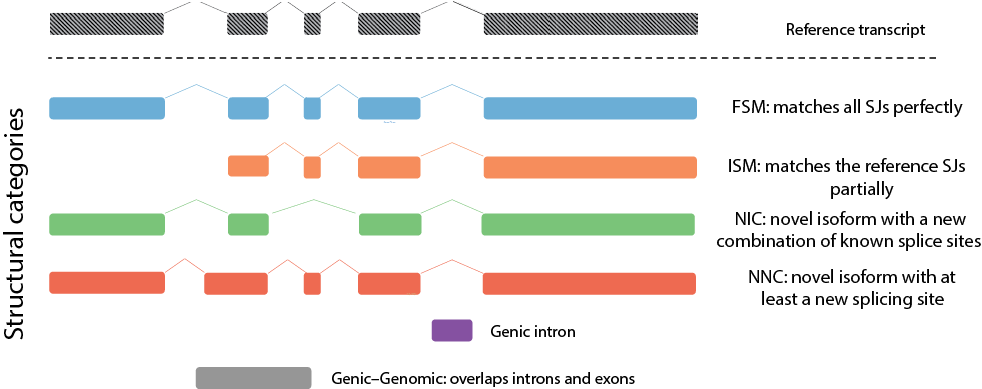
\includegraphics[width=\textwidth]{sqanti_structure_category.png}\\[0.2cm]
  {\scriptsize\emph{Source:} \href{https://www.nature.com/articles/s41592-024-02229-2}{Pardo-Palacios \emph{et al.}, 2024}}
\end{frame}

%--- Slides: QC Feature Blocks A–F --------------------------------------------------

% Block A -------------------------------------------------------------------------
\begin{frame}
  \frametitle{QC Feature Block A: Read-length \& Throughput (8 metrics)}
  \begin{table}[t]
    \centering
    \small
    \begin{tabular}{@{}ll@{}}
      \toprule
      No. & Metric \\
      \midrule
       1 & Mean read length \\
       2 & Median read length \\
       3 & Upper-quartile read length \\
       4 & Lower-quartile read length \\
       5 & \% reads $<\!$1 kb \\
       6 & \% reads 1--2 kb \\
       7 & \% reads 2--3 kb \\
       8 & \% reads $>\!$3 kb \\
      \bottomrule
    \end{tabular}
  \end{table}
  \vspace{0.4em}
  \begin{itemize}
    \item Captures depth and size bias to reveal degradation or protocol differences.
  \end{itemize}
\end{frame}

% Block B -------------------------------------------------------------------------
\begin{frame}
  \frametitle{QC Feature Block B: Read Structural Categories (8 metrics)}
  \begin{table}[t]
    \centering
    \small
    \begin{tabular}{@{}ll@{}}
      \toprule
      No. & Metric \\
      \midrule
       9  & \% Full-Splice-Match (FSM) reads \\
       10 & \% Incomplete-Splice-Match (ISM) reads \\
       11 & \% Novel-In-Catalog (NIC) reads \\
       12 & \% Novel-Not-in-Catalog (NNC) reads \\
       13 & \% Antisense reads \\
       14 & \% Fusion reads \\
       15 & \% Genic–genomic reads \\
       16 & \% Intergenic reads \\
      \bottomrule
    \end{tabular}
  \end{table}
  \vspace{0.4em}
  \begin{itemize}
    \item Describes transcript integrity and novelty at the single-read level.
  \end{itemize}
\end{frame}

% Block C -------------------------------------------------------------------------
\begin{frame}
  \frametitle{QC Feature Block C: UJC Structural Categories (8 metrics)}
  \begin{table}[t]
    \centering
    \small
    \begin{tabular}{@{}ll@{}}
      \toprule
      No. & Metric \\
      \midrule
       17 & \% FSM UJCs \\
       18 & \% ISM UJCs \\
       19 & \% NIC UJCs \\
       20 & \% NNC UJCs \\
       21 & \% Antisense UJCs \\
       22 & \% Fusion UJCs \\
       23 & \% Genic–genomic UJCs \\
       24 & \% Intergenic UJCs \\
      \bottomrule
    \end{tabular}
  \end{table}
  \vspace{0.4em}
  \begin{itemize}
    \item Collapses reads with identical junction chains, highlighting transcript-level novelty.
  \end{itemize}
\end{frame}

% Block D -------------------------------------------------------------------------
\begin{frame}
  \frametitle{QC Feature Block D: Splice-junction Quality (4 metrics)}
  \begin{table}[t]
    \centering
    \small
    \begin{tabular}{@{}ll@{}}
      \toprule
      No. & Metric \\
      \midrule
       25 & \% Known–canonical junctions \\
       26 & \% Known–non-canonical junctions \\
       27 & \% Novel–canonical junctions \\
       28 & \% Novel–non-canonical junctions \\
      \bottomrule
    \end{tabular}
  \end{table}
  \vspace{0.4em}
  \begin{itemize}
    \item Assesses splice-site accuracy—critical for long-read platforms.
  \end{itemize}
\end{frame}

% Block E -------------------------------------------------------------------------
\begin{frame}
  \frametitle{QC Feature Block E: Error / Artefact Flags (3 metrics)}
  \begin{table}[t]
    \centering
    \small
    \begin{tabular}{@{}ll@{}}
      \toprule
      No. & Metric \\
      \midrule
       29 & \% Reads with RT-switching repeat \\
       30 & \% Reads with intrapriming signature \\
       31 & \% Reads containing $\ge$1 non-canonical junction \\
      \bottomrule
    \end{tabular}
  \end{table}
  \vspace{0.4em}
  \begin{itemize}
    \item Flag well-known long-read artefacts to aid filtering.
  \end{itemize}
\end{frame}

% Block F -------------------------------------------------------------------------
\begin{frame}
  \frametitle{QC Feature Block F: Coverage \& Complexity (4 metrics)}
  \begin{table}[t]
    \centering
    \small
    \begin{tabular}{@{}ll@{}}
      \toprule
      No. & Metric \\
      \midrule
       32 & Total mapped read count \\
       33 & Mean reads per gene \\
       34 & Mean reads per UJC \\
       35 & Genes with $\ge$1 FSM read \\
      \bottomrule
    \end{tabular}
  \end{table}
  \vspace{0.4em}
  \begin{itemize}
    \item Summarises usable expression breadth and sequencing efficiency.
  \end{itemize}
\end{frame}

%--- Example: PCA on QC Features --------------------------------------------
\begin{frame}
  \frametitle{Example: PCA on QC Features}
  \begin{columns}[T]
    \begin{column}{0.55\textwidth}
      \centering
      \includegraphics[width=0.9\textwidth]{figures/Genome Res_figure2_a.jpg}
    \end{column}
    \begin{column}{0.4\textwidth}
      \small
      \textbf{Key insights from PCA:}
      \begin{itemize}
        \item Samples cluster by \textbf{sequencing technology}
        \item PC1 (56\%) separates \textcolor{green!60!black}{\textbf{cDNA ONT}} from \textcolor{blue}{\textbf{dRNA ONT}} and \textcolor{longtrec-orange}{\textbf{cDNA PacBio}}
        \item PC2 (35\%) separates \textcolor{blue}{\textbf{dRNA ONT}} from \textcolor{longtrec-orange}{\textbf{cDNA PacBio}}
        \item Clear technology-specific biases
        \item Enables outlier detection within technology groups
      \end{itemize}
      
      \vspace{0.3cm}
      \scriptsize
    \end{column}
  \end{columns}
\end{frame}

%--- Check-in Questions: SQANTI-reads Features -----------------------------
\begin{frame}
  \frametitle{Check-in Questions: SQANTI-reads Features}
  \begin{enumerate}
    \item What is the difference between analyzing reads versus UJCs (Unique Junction Chains)?
    \vspace{0.5cm}
    \item Which SQANTI3 structural categories would you expect to see more of in high-quality vs. low-quality samples?
    \vspace{0.5cm}
    \item Why might the percentage of FSM (Full-Splice-Match) reads be an important QC metric?
    \vspace{0.5cm}
    \item How could SQANTI-reads help you identify problematic samples in a multi-sample experiment?
  \end{enumerate}
\end{frame}

%%%%% SECTION: Case Studies
\section{Case Studies}

\begin{frame}
  \frametitle{LRGASP WTC11: Experimental Design}
  \centering
  % TikZ schematic centred in the slide
  \begin{tikzpicture}[every node/.style={font=\scriptsize, align=center}, node distance=0.8cm and 1cm]
    % ------------------------------------------------------------------
    % Technology boxes (top row)
    \node[draw, rounded corners, fill=longtrec-orange!35, minimum width=2.5cm, minimum height=0.8cm] (pacbio) {cDNA PacBio\\(n=3)};
    \node[draw, rounded corners, fill=longtrec-blue!35, minimum width=2.5cm, minimum height=0.8cm, right=of pacbio] (cdnaont) {cDNA ONT\\(n=3)};
    \node[draw, rounded corners, fill=green!35, minimum width=2.5cm, minimum height=0.8cm, right=of cdnaont] (drnaont) {dRNA ONT\\(n=3)};

    % QC metrics box (below technology boxes)
    \node[draw, rounded corners, fill=gray!20, minimum width=2.8cm, minimum height=1.0cm, below=of cdnaont] (qc) {35+\\SQANTI-reads\\metrics};

    % PCA box (bottom)
    \node[draw, rounded corners, fill=purple!25, minimum width=2.5cm, minimum height=1.0cm, below=of qc] (pca) {PCA\\scores \\+ loadings};

    % ------------------------------------------------------------------
    % Arrows
    \draw[->, thick] (pacbio.south) to[out=-90,in=180] (qc.west);
    \draw[->, thick] (cdnaont.south) -- (qc.north);
    \draw[->, thick] (drnaont.south) to[out=-90,in=0] (qc.east);
    \draw[->, thick] (qc.south) -- (pca.north);
  \end{tikzpicture}

  % ------------------------------------------------------------------
  % Annotation text (below figure, small font)
  \vspace{0.4em}
  {\scriptsize
  Triplicate transcriptome measurements of the WTC11 human cell line. Three long-read sequencing (LRS) library types were compared: cDNA PacBio Sequel II (cDNA PacBio), cDNA Oxford Nanopore MinION (cDNA ONT), Direct-RNA Oxford Nanopore MinION (dRNA ONT).}
\end{frame}

% Slide: PCA scores ---------------------------------------------------------
\begin{frame}
  \frametitle{PCA Scores: Technologies Form Distinct Clusters}
  \begin{itemize}
    \item PC1 (56\% variance) separates \textbf{cDNA ONT} from PacBio and dRNA ONT.
    \item PC2 (35\%) further discriminates \textbf{dRNA ONT} from \textbf{cDNA PacBio} libraries.
    \item Clear clustering indicates technology-specific QC signatures.
  \end{itemize}
  \vfill
  \centering
  \includegraphics[width=0.55\textwidth]{Genome Res_figure2_a.jpg}
\end{frame}

% Slide: PCA loadings -------------------------------------------------------
\begin{frame}
  \frametitle{PCA Loadings: Drivers of Variance}
  \begin{itemize}
    \item High \textbf{positive} PC1 loadings: total number of reads, \% NNC reads, and \% UJCs in the NNC category.
    \item High \textbf{negative} PC1 loadings: Intergenic and Genic–Genomic reads.
    \item PC2 is dominated by read-length metrics (1–2 kb, 2–3 kb, $>3$~kb).
  \end{itemize}
  \vspace{0.3cm}
  \centering
  \begin{columns}[c]
    \column{0.3\textwidth}
      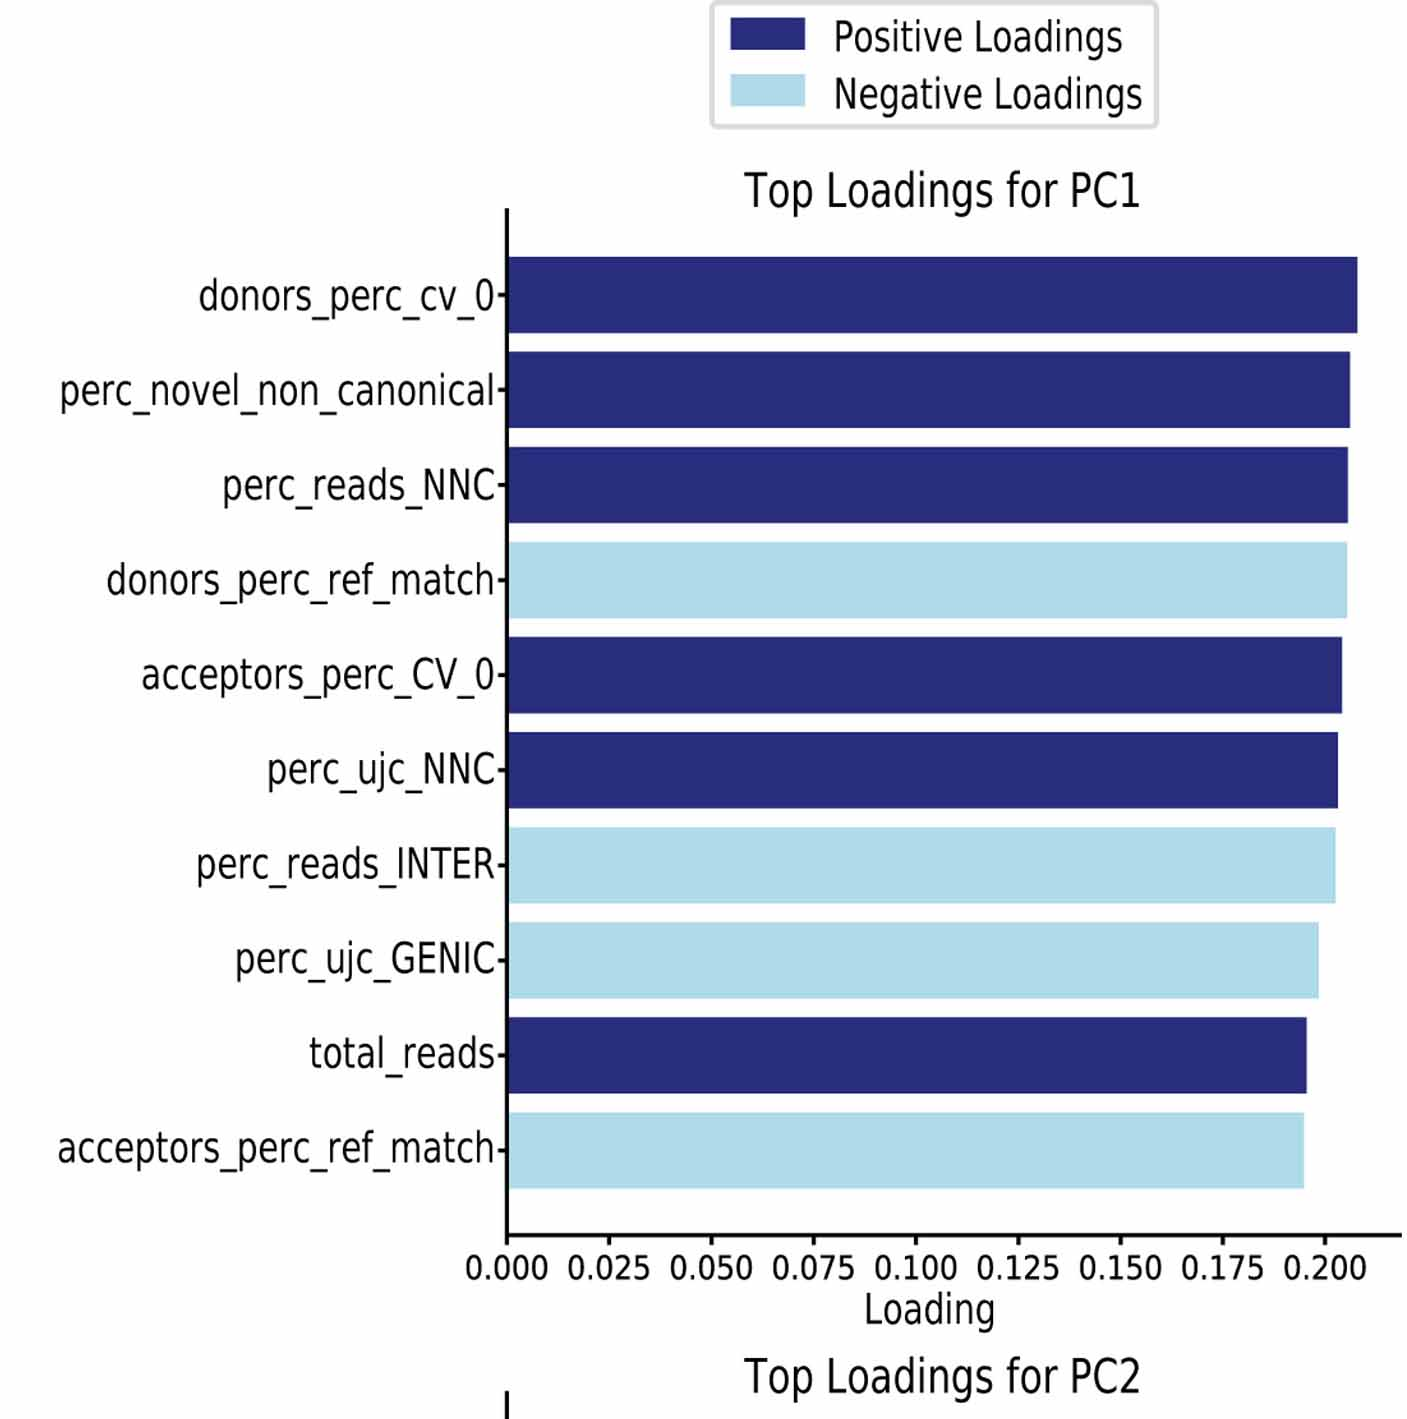
\includegraphics[width=\linewidth]{Genome Res_figure2_b1.jpg}
    \column{0.3\textwidth}
      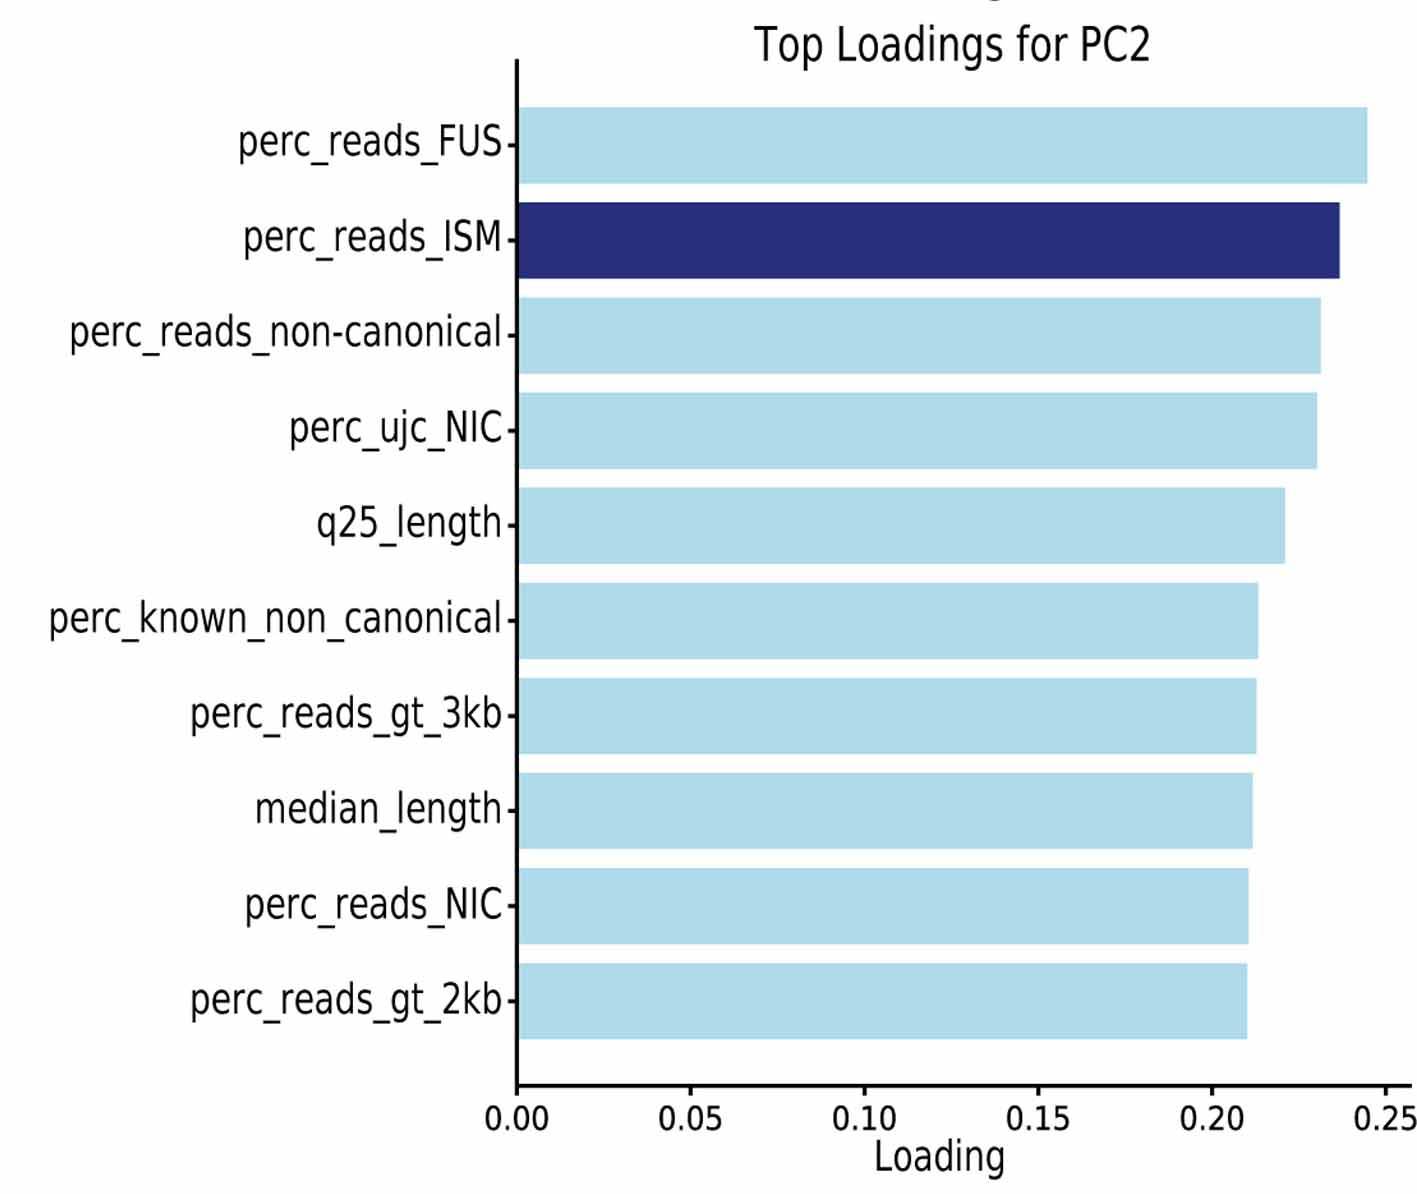
\includegraphics[width=\linewidth]{Genome Res_figure2_b2.jpg}
  \end{columns}
\end{frame}

%--- New Slide: Unique Junction Chain differences -----------------------------------
\begin{frame}
  \frametitle{UJC Profiles Differ by Technology}
  \begin{itemize}
    \item \textbf{cDNA ONT} libraries show the highest proportion of \textbf{NNC UJCs}.
    \item \textbf{dRNA ONT} and \textbf{cDNA PacBio} display lower UJC novelty, mirroring their lower NNC read fractions.
    \item Reinforces PCA PC1 loadings that highlight splice-junction novelty as a driver of variance.
  \end{itemize}
  \vspace{0.3cm}
  \centering
  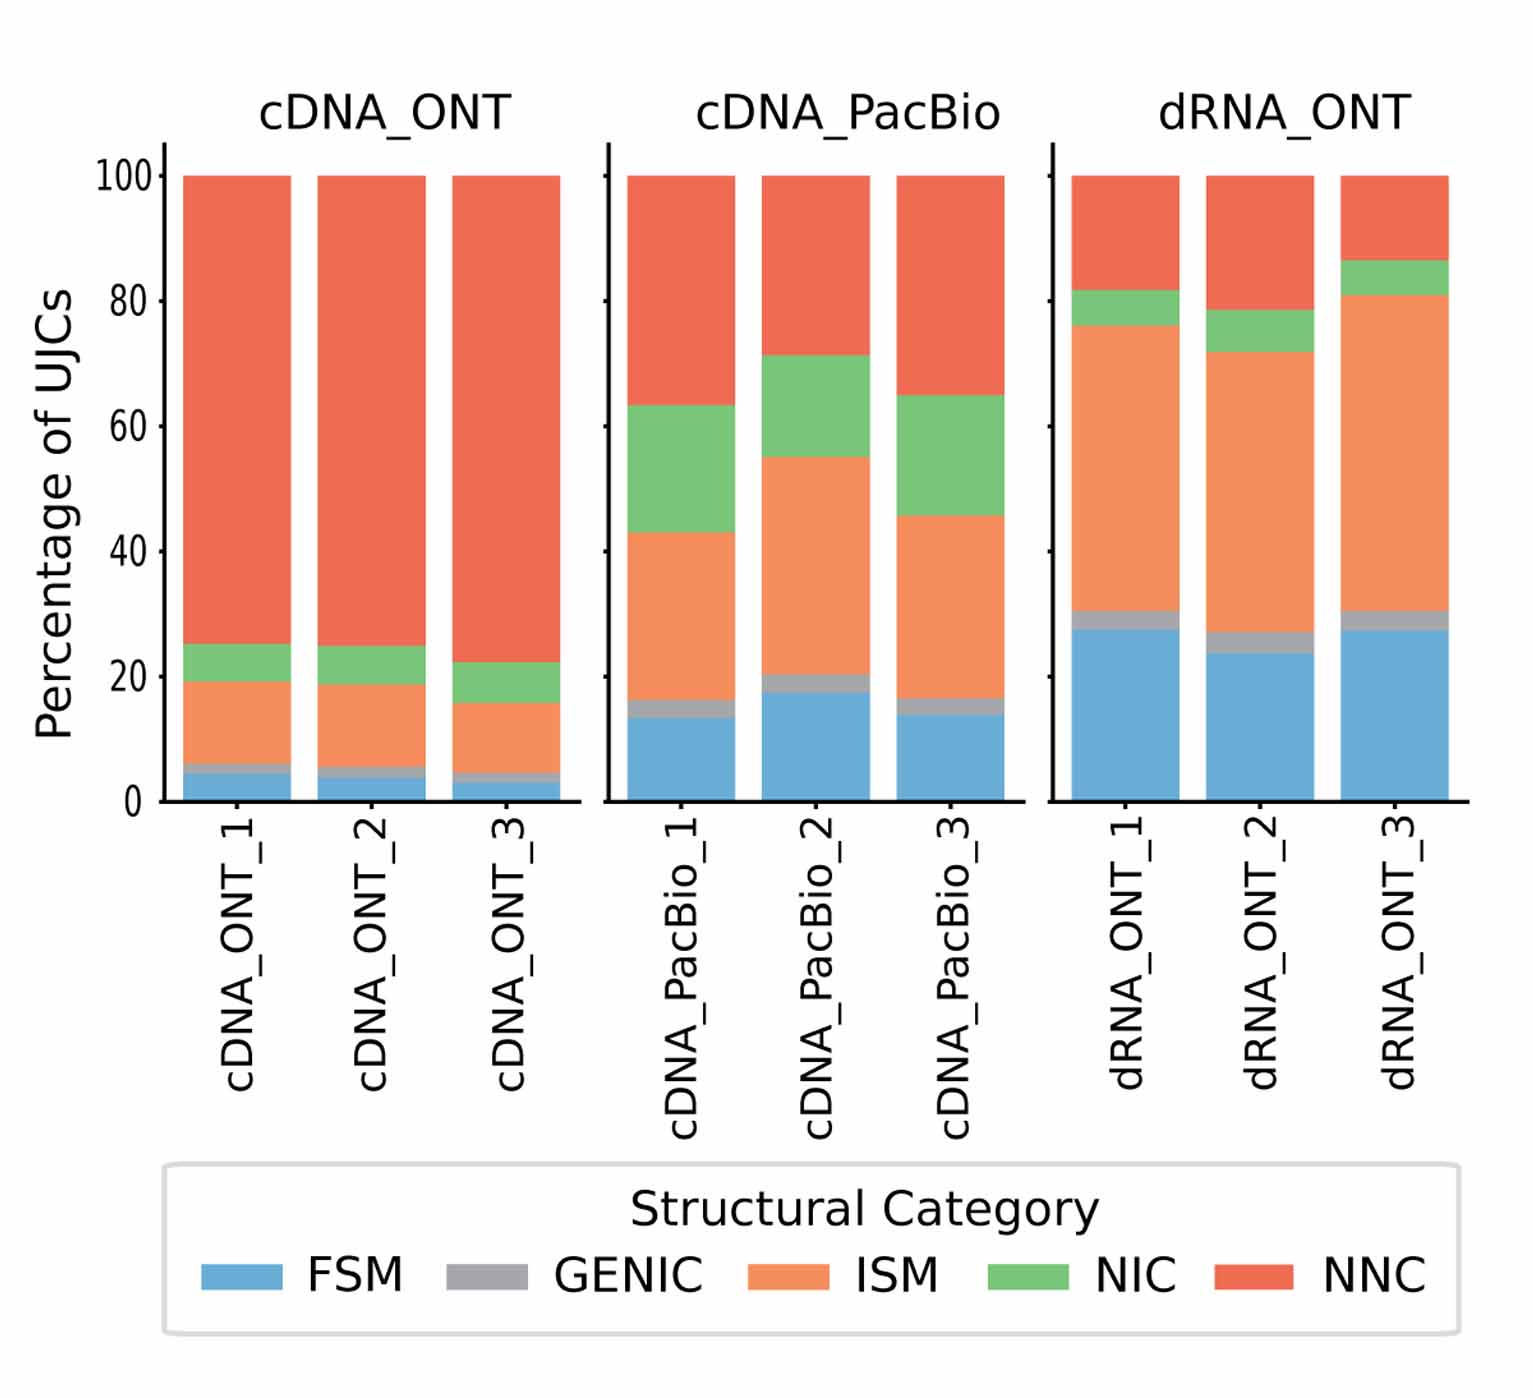
\includegraphics[width=0.35\textwidth]{Genome Res_figure2_d.jpg}
\end{frame}

% Slide: Structural category differences -----------------------------------
\begin{frame}
  \frametitle{Structural Category Profiles Differ by Technology}
  \begin{itemize}
    \item \textbf{cDNA ONT} exhibits the highest proportion of NNC reads and UJCs.
    \item \textbf{cDNA ONT} also shows the lowest fraction of intergenic reads.
    \item Confirms PC1 loadings and underscores library-prep biases.
  \end{itemize}
  \vspace{0.3cm}
  \centering
  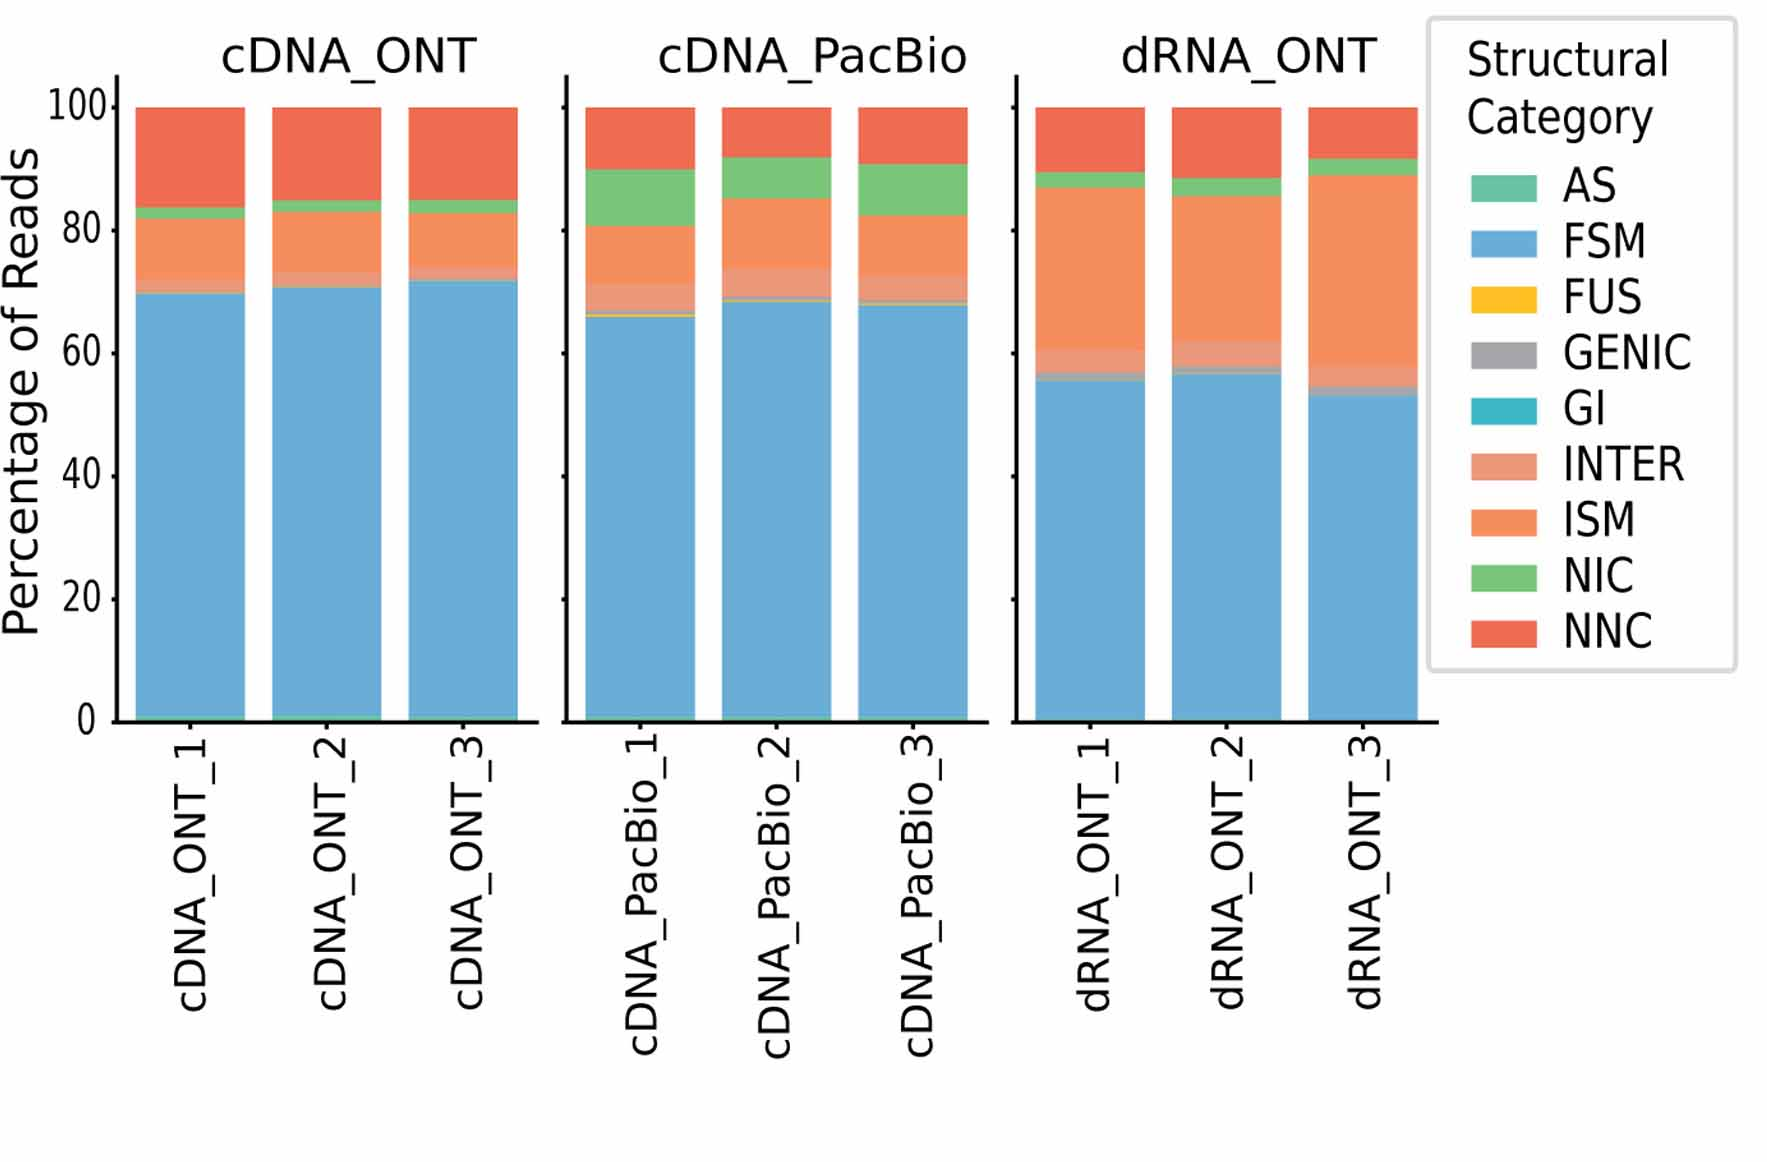
\includegraphics[width=0.5\textwidth]{Genome Res_figure2_c.jpg}
\end{frame}

% Slide: Read-length distributions -----------------------------------------
\begin{frame}
  \frametitle{Read-length Distributions Explain PC2 Separation}
  \begin{itemize}
    \item \textbf{cDNA PacBio} enriched for longer reads (1–2 kb, 2–3 kb, higher than 3 kb).
    \item \textbf{dRNA ONT} dominated by reads $<1$~kb.
    \item Aligns with strong read-length contributions to PC2.
  \end{itemize}
  \vspace{0.3cm}
  \centering
  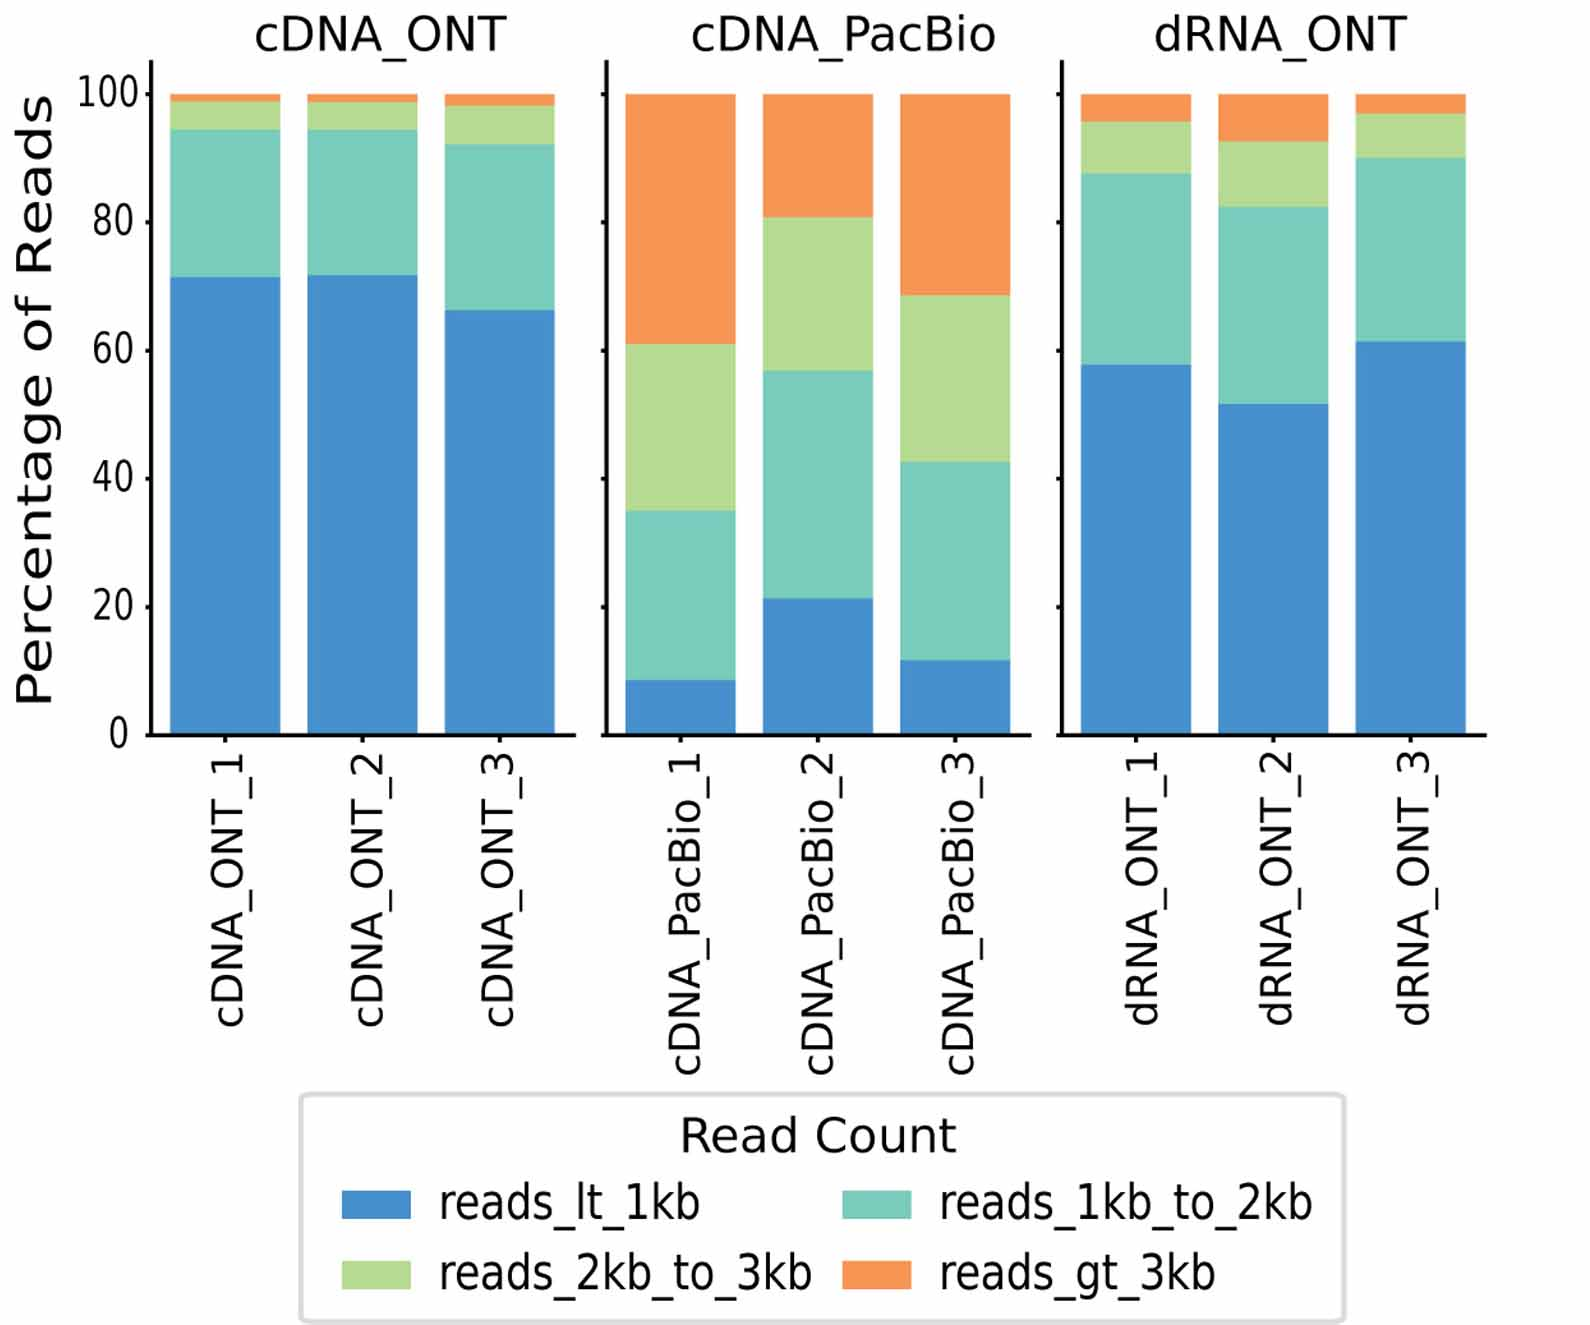
\includegraphics[width=0.4\textwidth]{Genome Res_figure2_e.jpg}
\end{frame}

% Slide: Take-aways -----------------------------------------------------------
\begin{frame}
  \frametitle{Take-aways: Drosophila Time-course}
  \begin{itemize}
    \item \texttt{SQANTI-reads} metrics facilitate depth-normalised sample comparison in multisample lrRNA-seq experiments.
    \item Short reads inflate ISM fraction, signalling RNA degradation.
    \item UJC and gene-level counts remain stable; higher depth boosts quantitative power.
    \item Integrated metric view readily pinpoints outlier libraries for removal prior to downstream analysis.
  \end{itemize}
\end{frame}

%--- Check-in Questions: Case Studies --------------------------------------
\begin{frame}
  \frametitle{Check-in Questions: Case Studies}
  \begin{enumerate}
    \item In the LRGASP WTC11 study, what did PC1 and PC2 represent, and why were they informative?
    \vspace{0.5cm}
    \item Why did cDNA ONT libraries show the highest proportion of NNC reads and UJCs?
    \vspace{0.5cm}
    \item How did read-length distributions help explain the separation between technologies?
    \vspace{0.5cm}
    \item What would you conclude if you saw a sample that clustered away from its expected technology group in PCA?
  \end{enumerate}
\end{frame}

%%%%% SECTION: Summary
\section{Summary}

% Slide: Take-home Messages (1/2)
\begin{frame}
  \frametitle{Take-home Messages \textnormal{(1/2)}}
  \begin{itemize}
    \item \textbf{Multi-sample dashboards}: stacked bars, heatmaps and ridgeplots instantly reveal QC metric trends across libraries.
    \item \textbf{PCA explorer}: interactive scores \& loadings plots pinpoint outliers, batch effects and technology biases.
    \item \textbf{Structural maps}: side-by-side visualisation of Unique Junction Chains and SQANTI3 categories clarifies read novelty.
    \item One-click toggle between \emph{reads}, \emph{UJCs} and \emph{gene}-level views—all colour-coded with the SQANTI3 palette.
  \end{itemize}
\end{frame}

% Slide: Take-home Messages (2/2)
\begin{frame}
  \frametitle{Take-home Messages \textnormal{(2/2)}}
  \begin{itemize}
    \item \textbf{Donor/Acceptor lollipops} and CV heatmaps spotlight weak splice sites with pixel-perfect resolution.
    \item \textbf{Under-annotation radar}: decision-tree badges and UpSet diagrams flag genes with putative novel isoforms.
    \item Exports as self-contained \textbf{HTML reports} for interactive sharing, or high-res PDF/SVG for publications.
    \item Designed for lectures and manuscripts—drop-in figures carry consistent fonts, colours and vector quality.
  \end{itemize}
\end{frame}

% References slide automatically generated from BibLaTeX database
\begin{frame}{References}
  \scriptsize
  % Print all entries from references.bib, even if not explicitly cited
  \nocite{*}
  \printbibliography[heading=none]
\end{frame}

% Thank you slide
\thankyouframe{Questions? Reach out at:}{https://longtrec.eu}{tianyuan.liu@csic.com}

\end{document} 